\chapter{Introduction}
\label{chapter:introduction}

20 years after its birth, the Web has become one of the defining
technological innovations that knows no geographical, political, or
ideological boundaries. The world wide platform built on top of the
physical Internet is deeply integrated into our daily lives. This
powerful tool that was built on egalitarian principles is now taken
for granted, just like old innovations such as
electricity. \cite{berners2010long}

In parallel with the rapid growth of the Web, mobile phones have
evolved from briefcase-sized ``portable'' telephony devices into
modern pocket-sized computers. The mobile revolution has already
changed the world as we see it, and more people have access to the Web
from a mobile device than from an Internet-connected desktop
computer. \cite{fling2009mobile}

The Web is not constrained into (desktop and laptop) computers and
mobile phones, though. Tablets, TVs, ebook readers, watches, and even
household appliances are connecting to the Internet and have web
browsers. For the first time in history, we have a truly ubiquitous
digital medium. \cite{fling2009mobile}

Universal accessibility and openness are the keys to being the
ubiquitous information platform of the digital age
\cite{berners2010long}. For the first time the Web truly accomplishes
its original principles in equality and universality; anyone can
access the vast source of open information from anywhere, with any
device. All you need is a web browser that supports the open standards
of the Web.

\begin{quotation}
  \noindent \textit{The goal of the Web is to serve humanity.}
  \begin{flushright}
    -- Tim Berners-Lee \cite{berners2010long}
  \end{flushright}
\end{quotation}

\begin{quotation}
  \noindent \textit{Not only does the majority of the mobile community
    believe that the mobile web is the future of the mobile medium,
    but I've also found it to have the highest return on investment,
    be it in terms of money, user satisfaction, or development time.}
  \begin{flushright}
    -- Brian Fling \cite{fling2009mobile}
  \end{flushright}
\end{quotation}

\section{Smartphone Landscape}
\label{section:smartphone-landscape}

\begin{table}
  \begin{tabular}{ l | l }
    \textbf{Mobile OS Type} & \textbf{Skill Set Required} \\
    \hline
    Apple iOS & C, Objective C \\
    Google Android & Java (Harmony flavored, Dalvik VM) \\
    RIM BlackBerry & Java (J2ME flavored) \\
    Symbian & C, C++, Python, HTML/CSS/JS \\
    Windows Mobile & .NET \\
    Windows 7 Phone & .NET \\
    HP Palm webOS & HTML/CSS/JS \\
    MeeGo & C, C++, HTML/CSS/JS \\
    Samsung bada & C++
  \end{tabular}
  \label{table:native-skills}
  \caption{Required skill sets for different mobile platforms. \cite{charland2011mobile}}
\end{table}

\section{HTML5}
\label{section:html5}

\subsection{History}
\subsection{Markup}
\subsection{CSS3}
\subsection{JavaScript APIs}
\subsection{Related APIs}

\section{Modern Mobile Web Application Architecture}
\label{section:modern-mobile-web}

\begin{figure}[ht]
  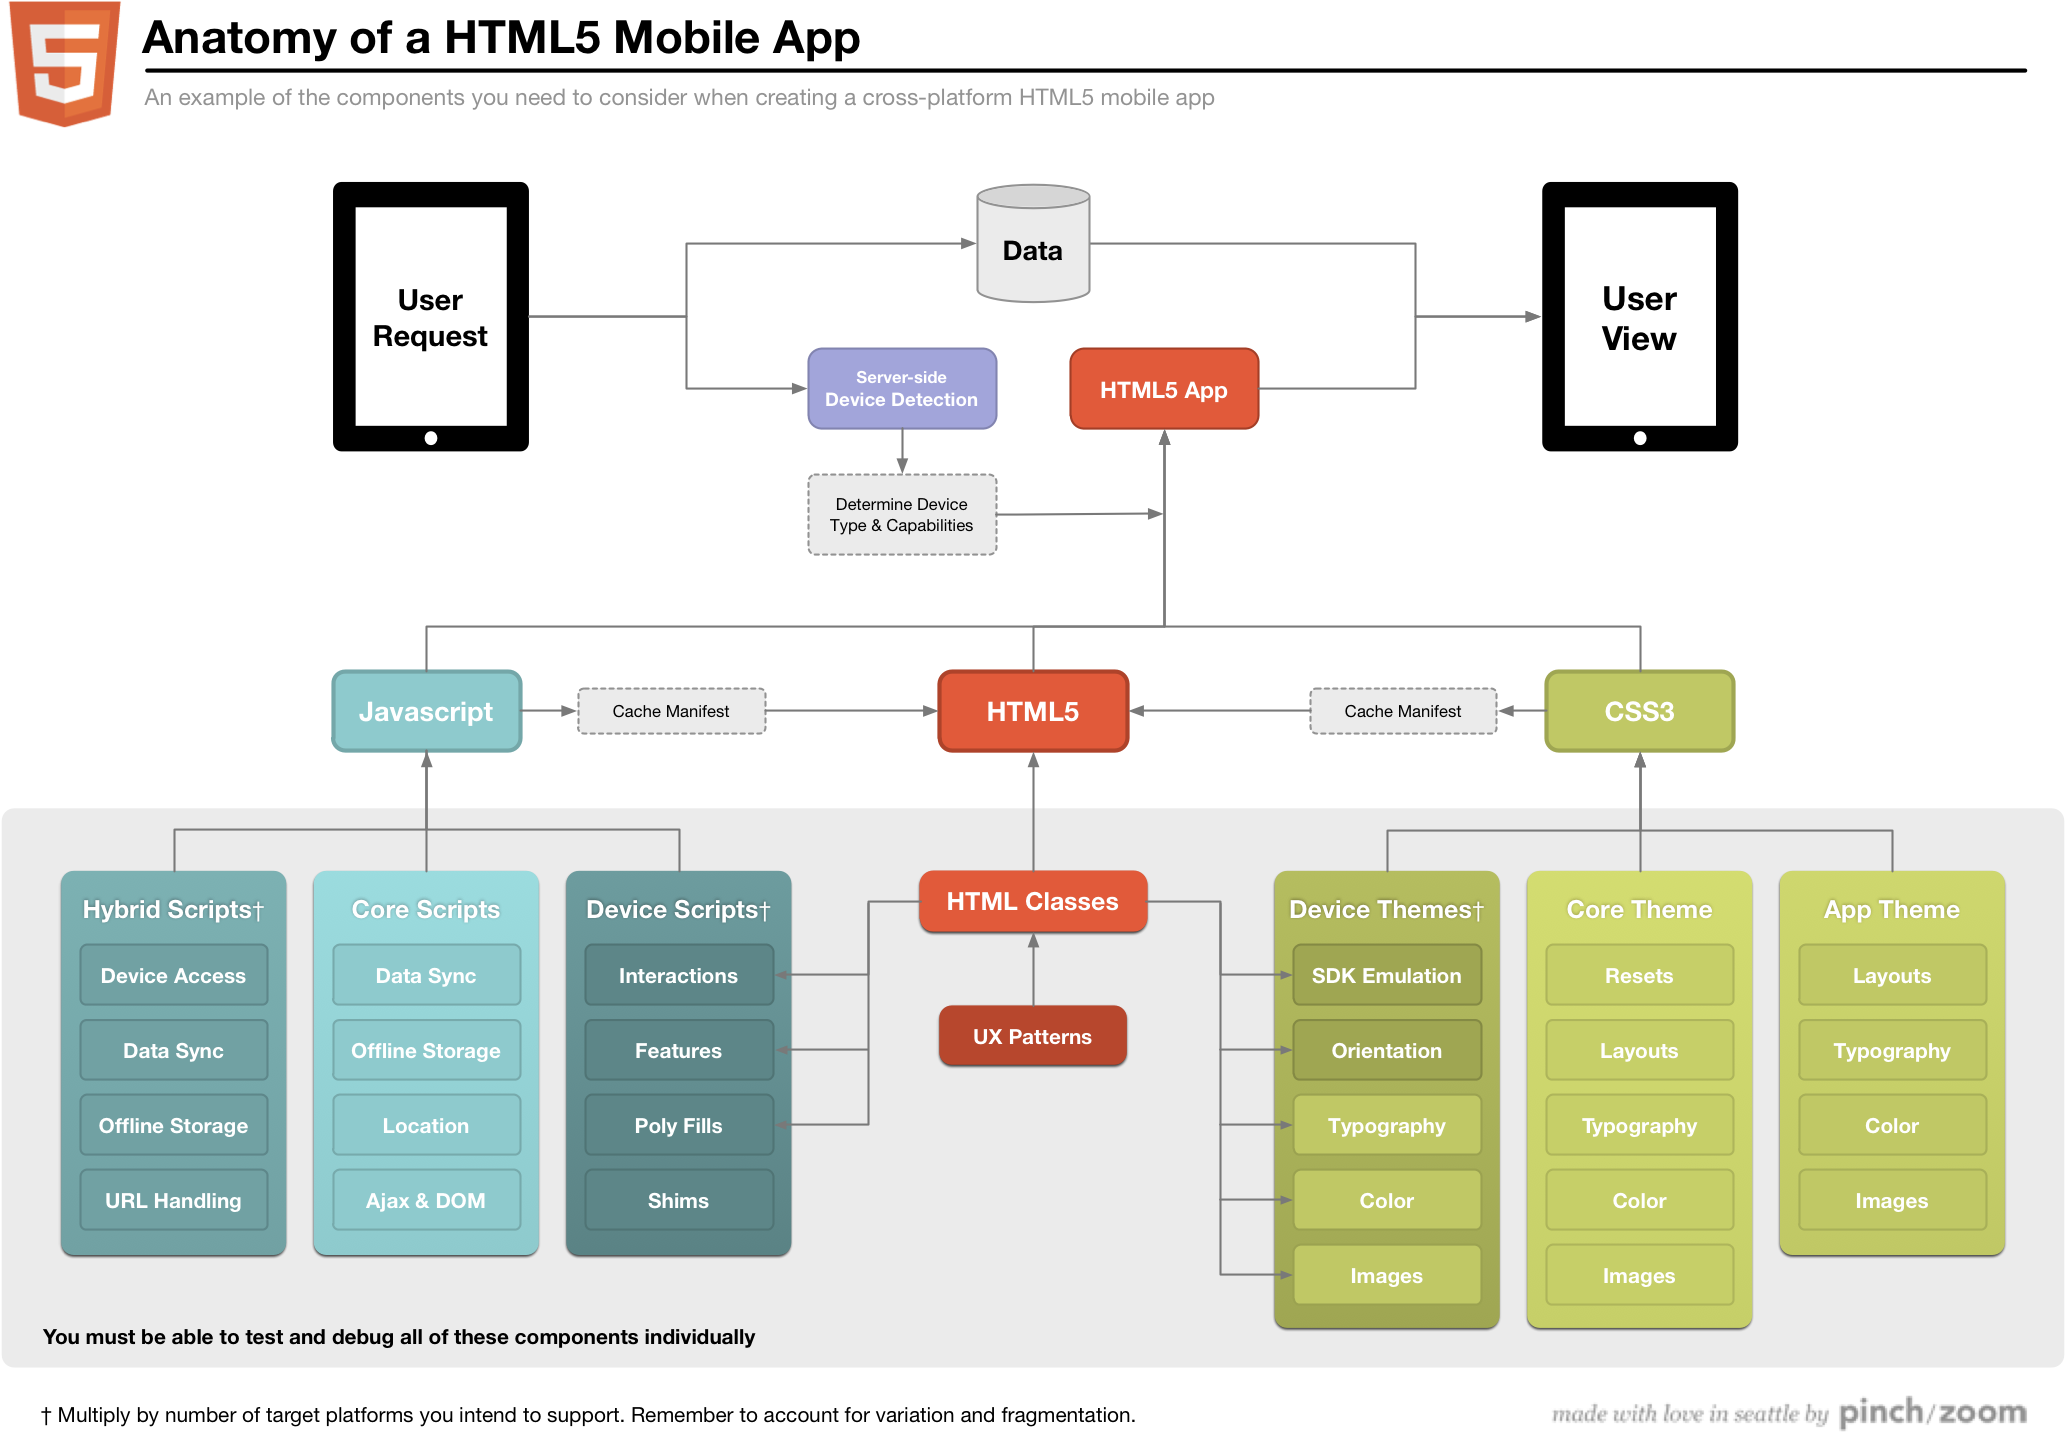
\includegraphics[width=\textwidth]{images/anatomy-of-a-html5-mobile-app.png}
  \caption{HTML5 Mobile Application Anatomy \citationneeded}
  \label{figure:anatomy-of-a-html5-mobile-app.png}
\end{figure}

\subsection{Single-Page applications}
\subsubsection{JavaScript MVC Libraries}

\subsection{Responsive Design}
\subsection{Progressive Enhancement}
\label{subsection:progressive-enhancement}

\subsection{UI Libraries}
\subsubsection{jQuery Mobile}
\subsubsection{jQTouch}
\subsubsection{Sencha Touch}

\subsection{Hybrid Applications}
\subsection{Wrapping Web Applications Application Stores}

\clearpage
\section{Performance Guidelines}
\label{section:performance-guidelines}

There are several web application performance best practices and
related guidelines. According to Souders \cite{souders2007high}, only
10--20\% of the end user response time is spent generating and
transferring the HTML document from the web server to the
client. Therefore, most of the optimization should be done in the
frontend for best improvement opportunities. Below we list the
performance guidelines defined by Souders \cite{souders2007high,
  souders2009even}.

\begin{itemize}

  % High Performance Web Sites

\item \textbf{Make Fewer HTTP Requests}

  According to Souders, 80--90\% of the end user response time is
  spent downloading components in a page other than the requested HTML
  page. Therefore, the simplest way to improve the response time is to
  reduce the number of HTTP requests needed to get all the required
  components.

  There are several ways to reducing the number of needed HTTP
  requests. Combining images into sprites, inlining images, or
  combining separate JavaScript and CSS files result in fewer
  components needed to download in a page.

\item \textbf{Use a Content Delivery Network}

  As web applications are deployed and become accessible worldwide,
  latency might become an issue for users far from the application's
  web servers. Geographically distributed servers allow for serving
  the application as close to the user as possible.

\item \textbf{Add an Expires Header}

  Avoiding a HTTP request altogether is the best option for reducing
  the response time when downloading the components in a page. Good
  caching strategies help browsers to know which resources are valid
  and for how long until they should be updated.

  The Expires header in HTTP tell the client how long a resource is
  valid, and especially far future Expires headers reduce the need for
  downloading an updating the components in a page after the initial
  download.

\item \textbf{Gzip Components}

  Compressing HTTP responses is an easy and effective way to reduce
  the size of the data needed to transfer across the
  network. Compression is supported widely in web browsers and the
  impact of reduced response sizes is huge. Using Gzip, the response
  size is reduced generally about 70\%.

\item \textbf{Put Stylesheets at the Top}

  Putting the CSS files to the top of the document allows the page to
  load progressively and the browser show visual feedback to the user
  as early as possible.

\item \textbf{Put Scripts at the Bottom}

  Because scripts block parallel downloads, they should be included to
  the page after all other resources. They also block progressive
  rendering of all content below them in the HTML document, and should
  therefore be at the bottom of the document.

\item \textbf{Avoid CSS Expressions}

  CSS expressions are a way to dynamically set CSS properties in
  Internet Explorer by evaluating a JavaScript code in a
  stylesheet. However, despite the obvious upsides, the expressions
  are evaluated at such a high frequency that they negatively impact
  the performance.

\item \textbf{Make JavaScript and CSS External}

  There are performance tradeoffs between making JavaScript and CSS
  external versus inlining them in the HTML document. In the typical
  case, however, making them external enables the browser to leverage
  the HTTP caching semantics and thus reduces the needed network
  transfer.

\item \textbf{Reduce DNS Lookups}

  Apart from cached DNS lookups, the browser typically needs 20--120
  milliseconds to look up the \abbr{IP} address for a given
  hostname. The cache lifetime of a lookup depends on the \abbr{TTL}
  value of the DNS record and having the components of a page
  distributed across several domains might accumulate into a
  noticeable response time.

  There is also a trade off between unique hostnames and allowed
  parallel connections and therefore these settings should be
  configured based on the application architecture and needs.

\item \textbf{Minify JavaScript}

  Because JavaScript is an interpreted language that must be sent to
  the web browser as source code, minifying the code reduces the
  required network transfer. Minifiers and obfuscators optimize the
  size of the source code by stripping extra whitespace and comments
  as well as renaming variable and function names to shorter ones
  without changing the interpreted behavior of the code.

\item \textbf{Avoid Redirects}

  Rerouting any component in a page takes time, and avoiding any kind
  of redirects improves the response times.

\item \textbf{Remove Duplicate Scripts}

  Including a resource several times serves no purpose but is actually
  quite common. Developers should make sure to include resources only
  once.

\item \textbf{Configure ETags}

  \abbr{ETags} are a mechanism in HTTP for servers and browsers to
  validate cached resources. The typical default values set by
  commonly used web servers might hurt performance, and should thus be
  configured properly to address the application architecture and
  needs.

\item \textbf{Make Ajax Cacheable}

  Highly dynamic web sites have a lot of \abbr{Ajax} functionality,
  and developers should make sure all the requested URLs for data
  fetching follow the performance best practices such as having the
  proper caching in place.

  % Even Faster Web Sites

\item \textbf{Splitting the Initial Payload}

  Nowadays, web sites include a lot of resources and JavaScript
  functionality, but only a small part of the downloaded components
  are used in the typical use cases of the application. Splitting the
  resources into bundles that can be lazily downloaded when first
  needed reduces the initial payload needed to transfer on application
  startup.

\item \textbf{Loading Scripts Without Blocking}

  Most browsers block the downloads of other resources when scripts
  are being downloaded and executed. There are several ways to
  circumvent this behavior to allow browsers download scripts in
  parallel with other resources as well as with other script files.

\item \textbf{Coupling Asynchronous Scripts}

  Related to the previous item, when using parallel downloads with
  scripts that are dependent on each other, race conditions might
  occur due to the varying order of download and execution. Therefore,
  asynchronous scripts dependent on each other should be coupled to
  preserve the correct order of execution.

\item \textbf{Positioning Inline Scripts}

  Inline scripts do not introduce a HTTP request, but they can still
  block parallel downloads of other resources and they might affect
  also the progressive rendering of the page. With the correct
  positioning of the scripts, these problems can be handled properly.

\item \textbf{Writing Efficient JavaScript}

  After networking, the obvious place to optimize the runtime speed of
  a web application is the JavaScript code.

  Because the whole \abbr{UI} and the JavaScript code run in the same
  browser thread, there can be only one thing happening at a
  time. Long running functions block the UI from updating and can
  result in bad \abbr{UX}.

  Splitting the running code into properly sized chunks, appropriately
  leveraging the asynchronous patterns of JavaScript in the
  application architecture, understanding the details and slow parts
  of the DOM API, and using several JavaScript programming best
  practices can result in big improvements in the perceived
  application performance. \cite{zakas2010high}

\item \textbf{Scaling with Comet}

  For real-time data-driven applications, there are various
  optimization techniques related to optimizing the constant data
  transfer between the server and the client. The collection of there
  various technologies is unofficially called Comet.

\item \textbf{Going Beyond Gzipping}

  Although Gzipping is widely supported in web browsers, there are
  cases when it is not supported or when the support is not
  indicated. Stripping extra content such as unneeded whitespace and
  comments reduces the payload size for uncompressed responses. There
  are also ways to detect Gzip support if the client does not directly
  indicate that.

\item \textbf{Optimizing Images}

  Images typically tend to account for a large portion of the page
  weight, and since the page weight is highly correlated to the
  response time, images are a natural target for optimization. There
  are several ways to optimize images either with lossy or lossless
  conversions.

\item \textbf{Sharding Dominant Domains}

  By tuning the amount of unique hostnames used for serving all the
  resources of an application, parallel downloads can be better
  leveraged. Also, by using HTTP 1.0 with proper Keep-Alive headers or
  HTTP 1.1 with proper persistent connections the parallel downloads
  can be tuned for better performance.

\item \textbf{Flushing the Document Early}

  Some web application frameworks allow flushing parts of the document
  to the user before the whole document is generated. This enables
  progressive rendering and gives faster feedback to the user and thus
  improves the perceived performance.

\item \textbf{Using Iframes Sparingly}

  Iframes enable developers to embed a separate HTML document inside
  another document. They are useful in sandboxing external documents
  in the same view, but the iframe element is the most expensive DOM
  element related to the page performance.

\item \textbf{Simplifying CSS Selectors}

  There are several ways to choose elements in CSS stylesheets to
  apply the defined properties to. Some selectors are faster than
  others and some have terrible performance.

\end{itemize}
